\documentclass[fr]{../../../eplsummary}

\usepackage{../../../eplunits}
\usepackage{../../../eplelec}
\usepackage{circuitikz}

\hypertitle{Circuits électroniques analogiques et digitaux fondamentaux}{5}{ELEC}{1530}
{Antoine Paris}
{Denis Flandre et Jean-Didier Legat}

\paragraph{Notations}
La synthèse suit la notation du livre et du cours.
Un signal $i_C(t)$ est réprésenté mathématiquement
comme ayant une composante constante $I_C$ et une
composante variable $i_c(t)$ de telle sorte que
\[ i_C(t) = I_C + i_c(t). \]
On utilise $I_c$ pour indiquer l'amplitude de
la composante variable $i_c(t)$. 

\part{Dispositifs et circuits de base}
\section{Amplificateurs opérationnels}
Voir synthèse du cours LELEC1370.

\section{Diodes}
\subsection{Diode idéale}
Idéalement, la diode se comporte comme un
interrupteur ouvert quand la tension à ses
bornes est négative et fermé dans le cas
contraire. Le symbole de la diode est quant
à lui donné à la figure \ref{fig:diode-reprensation}.
La courbe courant-tension de la diode idéale est
quant à elle représentée sur la
figure \ref{fig:iv-ideal-diode}. 

\begin{figure}[ht]
	\centering
	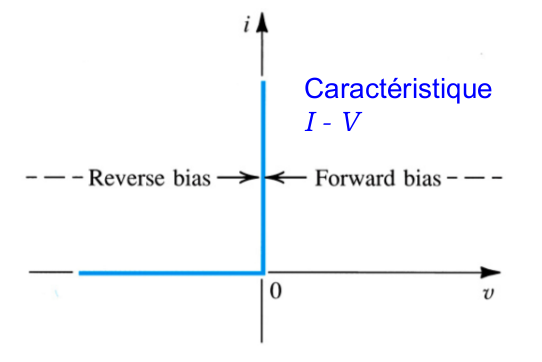
\includegraphics[scale=0.35]{img/iv-ideal-diode.png}
	\caption{Courbe caractéristique d'une diode idéale.}	
	\label{fig:iv-ideal-diode}
\end{figure}

\begin{figure}[ht]
	\centering
	\begin{circuitikz}[american voltages]
		\draw (0,0) to [diode, v^<=$v$, i_=$i$] (4,0); 
	\end{circuitikz}
	\caption{Symbole et conventions de sens pour la diode.
	L'anode est définie comme étant la partie polarisée
	positivement tandis que la cathode est définie comme
	la partie étant polarisée négativement.}
	\label{fig:diode-reprensation}
\end{figure}

Formellement, deux configurations sont possibles :
\begin{itemize}
	\item Bloquante (\textit{reverse bias}) : $v < 0 \Rightarrow i = 0$.
	La diode se comporte comme un circuit ouvert ;
	\item Passante (\textit{forward bias}) : $i > 0 \Rightarrow v = 0$.
	La diode se comporte comme un court-circuit.
\end{itemize}

\subsubsection{Application : le redresseur}
En appliquant directement le modèle idéal de la diode,
il apparaît immédiatement que le circuit de la figure
\ref{fig:redresseur} permet de ``couper`` la partie
négative du signal d'entrée $v_I$. Formellement,

\[
v_O = \begin{cases} 
v_I, & \mbox{si } v_I > 0 \\
0,   &\mbox{si } v_I < 0
\end{cases}.
\]

\begin{figure}[ht]
	\centering
	\begin{circuitikz}[american voltages]
		\draw (0,0) to [diode, v^<=$v_D$, i_=$i_D$] (4,0); 
		\draw (0,-2) to [american voltage source, v=$v_I$] (0,0);
		\draw (4,0) to [R, v^<=$v_O$] (4,-2);
		\draw (4,-2) to [short] (0,-2);
	\end{circuitikz}
	\caption{Circuit d'un redresseur.}
	\label{fig:redresseur}
\end{figure}

Cependant, en simulant ce circuit sur SPICE,
on se rend compte que le résultat ne correspond
pas exactement à celui attendu.

\subsection{Modèle empirique pour la diode réelle}
Plusieurs non-idéalités apparaissent en effet : un
décalage en tension en mode passant, un courant
non-nul et une tension de claquage en mode bloquant.
\`{A} haute fréquence, on remarque aussi une certaine
latence lorsque la diode passe du sens passant à bloquant.
D'un point de vue circuit, on représente donc une diode
réelle comme une source de courant en parallèle avec un
condensateur, le tout en série avec une résistance.
La courbe caractéristique d'une diode réelle est représentée
sur la figure \ref{fig:iv-real-diode}.

\begin{figure}[ht]
	\centering
	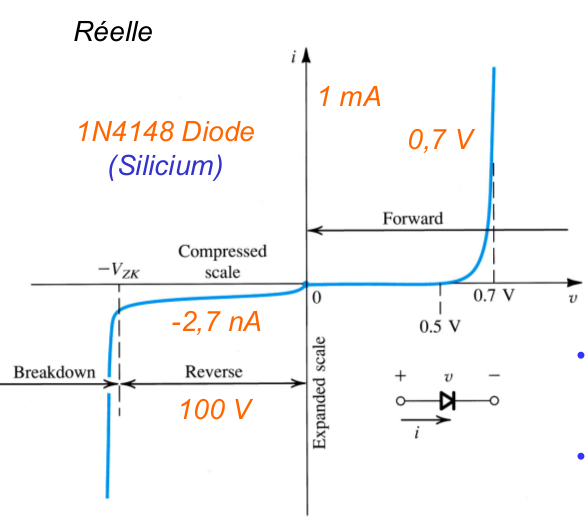
\includegraphics[scale=0.30]{img/iv-real-diode.png}
	\caption{Courbe caractéristique d'une diode réelle.}	
	\label{fig:iv-real-diode}
\end{figure}

En sens passant, on peut approximer le comportement
de la diode par un modèle à chute de tension constante,
dont la courbe caractéristique est représenté sur la
figure \ref{fig:iv-almost-ideal-diode}.

\begin{figure}[ht]
	\centering
	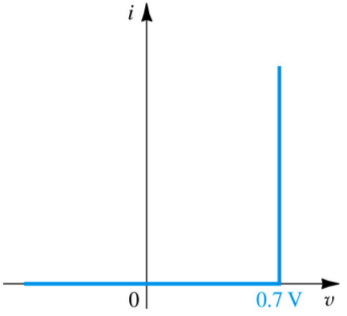
\includegraphics[scale=0.35]{img/iv-almost-ideal-diode.png}
	\caption{Courbe caractéristique d'une diode quasi-idéale.}	
	\label{fig:iv-almost-ideal-diode}
\end{figure}

De manière plus exacte, ce comportement en sens passant
est modélisé de manière empirique par l'équation
\[ i_D = I_S\left(e^{\frac{v_D}{n\cdot V_T}} - 1\right). \]
Dans cette équation, $n$ est constante empirique et
$V_T = \frac{k\cdot T}{q}$ est le coéfficient de température.
Son effet est représenté sur la figure \ref{fig:temp-effect-diode}.
\`{A} \SI{27}{\celsius}, $V_T = \SI{26}{\milli\volt}$.

\begin{figure}[ht]
	\centering
	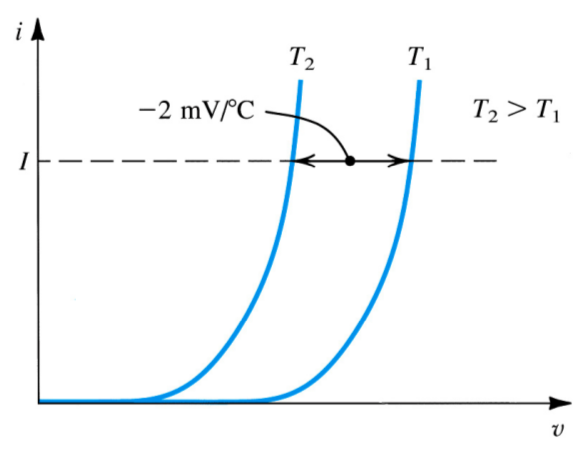
\includegraphics[scale=0.23]{img/temp-effect-diode.png}
	\caption{Effet de la température sur une diode.}	
	\label{fig:temp-effect-diode}
\end{figure} 

\subsection{Modèle petit signal}
\subsubsection{En général}
Soit un composant électronique dont la relation courant-tension
est donnée par une fonction $f$ non-linéaire telle que $i_D = f(v_D)$.
On peut décomposer $v_D$ en une composante constante $V_D$ et une
composante variable $v_d$ avec $v_d$ très petit.

La série de Taylor de $f(v_D)$ autour du point d'opération DC
$V_D$ est donnée par
\[ i_D = f(V_D) + \left. \frac{\dif f(v_D)}{\dif v_D}\right|_{v_D=V_D}\cdot v_d + \dots \]
où les termes d'ordre supérieurs peuvent être négligés car $v_d$ est
très petit. En décomposant $i_D$ en sa partie constante et sa
partie variable, on peut réecrire l'égalité précédente
\[ I_D + i_d \approx f(V_D) + \left. \frac{\dif f(v_D)}{\dif v_D}\right|_{v_D=V_D}\cdot v_d. \]
En égalant partie constante et partie variable de chaque côté,
on obtient finalement
\begin{align*} 
I_D &\approx f(V_D) \\ 
i_d &\approx \left. \frac{\dif f(v_D)}{\dif v_D}\right|_{v_D=V_D}\cdot v_d.
\end{align*}
On constate donc que la réponse $i_d$ au petit signal $v_d$
est maintenant une fonction linéaire de $v_d$. On défini 
$g_d = 1/r_d$ comme étant la conductance petit-signal
\[ g_d = \left. \frac{\dif f(v_D)}{\dif v_D}\right|_{v_D=V_D}.\]

Une interprétation graphique de ce raisonnement mathématique
est donnée à la figure \ref{fig:small-signal-method-graph}.

\begin{figure}[ht]
	\centering
	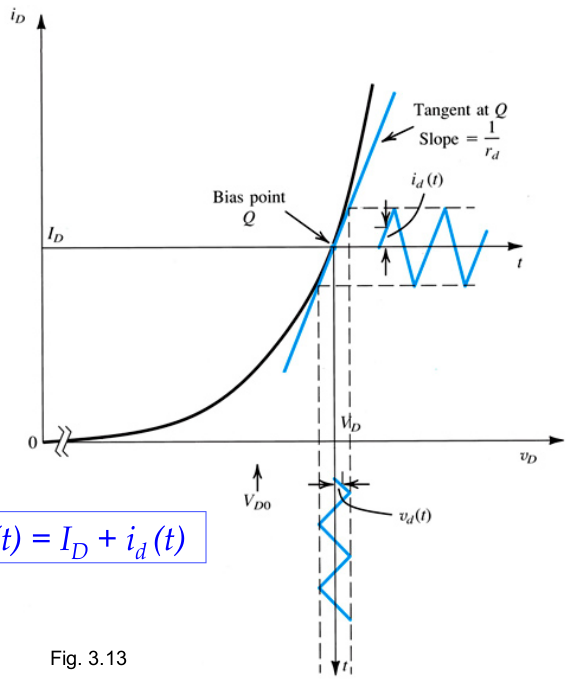
\includegraphics[scale=0.35]{img/small-signal-method-graph.png}
	\caption{Interprétation graphique de la méthode du petit signal.}	
	\label{fig:small-signal-method-graph}
\end{figure}

\subsubsection{Dans le cas de la diode}
Pour une diode, la relation non-linéaire est donnée par
\[ i_D(v_D) = I_s \cdot e^{v_D/V_T}. \] 
% FIX ME : Quid du -1 de la formule donnée plus haut?
En appliquant le même raisonnement que dans le cas général,
on trouve que la résistance petit-signal d'une diode
(aussi appelé sa résistance dynamique) est donnée par
\[ r_d = \frac{V_T}{I_D}. \]
Autrement dit, pour un signal suffisament petit, une
diode se comporte comme une résistance. On dit alors que
le modèle petit signal d'une diode est une résistance.
Il faut cependant faire attention à modifier ce modèle
petit-signal à haute fréquence pour prendre en compte
la capacité parasite de la diode.

% TODO : applications (half-wave-rectifier, full-wave-rectifier,
% peak-rectifier)

\subsection{Diode Zener}
Les diodes Zener sont plutôt utilisé en sens \textit{reverse}
pour avoir une tension de seuil plus élevé (de l'ordre de \SI{6.8}{\volt}).
Le symbole d'une diode Zener est donné à la figure
\ref{fig:diode-zener-representation}.

\begin{figure}[ht]
	\centering
	\begin{circuitikz}[american voltages]
		\draw (0,0) [zDo, v^>=$V_Z$, i_<=$I_Z$] to (4,0);
	\end{circuitikz}
	\caption{Symbole et conventions courant-tension pour une
	diode Zener.}
	\label{fig:diode-zener-representation}
\end{figure}

% TODO : à creuser un peu plus

\subsection{Diodes spéciales}
Une diode \textbf{Schottky} est une diode qui a un seuil de tension très bas
(de l'ordre de 0.3 à \SI{0.4}{\volt}) et un temps de commutation très
faible.

Une diode varicap (pour \textit{variable capacity}) ou  \textbf{varactor}
est une diode qui se comporte comme un condensateur variable.

Une \textbf{photodiode} permet quant à elle de transformer un rayonnement
du domaine optique en un signal électrique.

Enfin, une \textbf{diode électroluminescente} (LED pour
\textit{Light-Emmiting-Diode} en anglais) est une diode
capable d'émettre de la lumière lorsqu'elle est traversée par
un courant.

\section{MOSFET}
\subsection{Structure du transistor MOS}

\subsection{Caractéristiques courant-tension}

\end{document}
